\documentclass[10pt]{article}
\usepackage{parskip}
\usepackage[utf8]{inputenc}
\usepackage[left=2.00cm, right=2.00cm, top=2.00cm, bottom=2.00cm]{geometry}
\usepackage[spanish]{babel}
\usepackage{graphicx,subfig}
\usepackage{fancyhdr}
\graphicspath{{Imagenes/}}
\usepackage{enumerate} 
\usepackage{multicol}
\begin{document}


\pagestyle{fancy}
\cfoot{}


%Cabeceras
\rhead{Distribución de las cargas eléctricas}
\lhead{}

%Portada
\begin{titlepage}
	\newgeometry{
		left=25mm,
		right=25mm,
		top=5mm,
		bottom=30mm,
		headheight = 0 mm
	}

	\begin{figure}[t]
		\subfloat{
\includegraphics[width=0.15\textwidth]{Logo_IPN}}
		\hspace{0.6\textwidth}
		\subfloat{
\includegraphics[width=0.22\textwidth]{LogoEsime}}
	\end{figure}

	\centering
	{\bfseries\Huge Instituto Politécnico Nacional. \par}
	\vspace{1cm}
	{\scshape\Large Ingeniería en Comunicaciones y Electrónica. \par}
	\vspace{0.3cm}
	{\scshape\Large Laboratorio de Electricidad y Magnetismo.  \par}
	\vspace{1cm}
	{\scshape\Huge ECHALE TIERRA \par}
	\vspace{1cm}
	{\itshape\Large Distribución de las cargas eléctricas en los conductores. \par}
	{\Large 2CM13\par}
	\vfill
	{\Large Autores: \par}
	{\Large Daniela Elizabeth Pérez Vargas. \par}
	{\Large Jesús Martinez Amac. \par}
	{\Large José Emilio Hernández Huerta. \par}
	{\Large Nataly Bejarano Garduño..\par}
	{\Large Uriel Grimaldi Díaz.  \par}
	\vfill
	{\Large Abril 2023. \par}

\end{titlepage}

\tableofcontents
\newpage




\section{Resumen.}
Por medio de los materiales proporcionados en el laboratorio de la escuela, los alumnos realizaron experimentos con relacion a la distribucion de cargas en los conductores, siendo especificos realizaron estos experimentos con la ayuda de un generador Vander Graff, un electroscopio y diversos materiales más. Para llegar a tener las conclusiones necesarias para entender los conceptos basicos de electricidad y magnetismo.

\begin{multicols}{2}
\section{Objetivo.}
El alumno determinara mediante instrumentacion si un cuerpo esta cargado al igual de su polaridad, con las Experiencias de Cavendish y Franklin verificaran la carga electrica que se distrubuye en en la superficie exterior, razonaran el porque dentro de un conductor electrico hueco el campo electrico es nulo. Y para finalizar explicaran lo que sucede con el efecto puntas al realizar las experiencias del rejilete, la bujia y el mechon de cabello.

\section{Introducción.}



\section{Marco teórico.}



\section{Descripción de materiales.}

 Generador de van der Graff: sirve para acumular gran cantidad de carga eléctrica dentro de su esfera hueca.
 
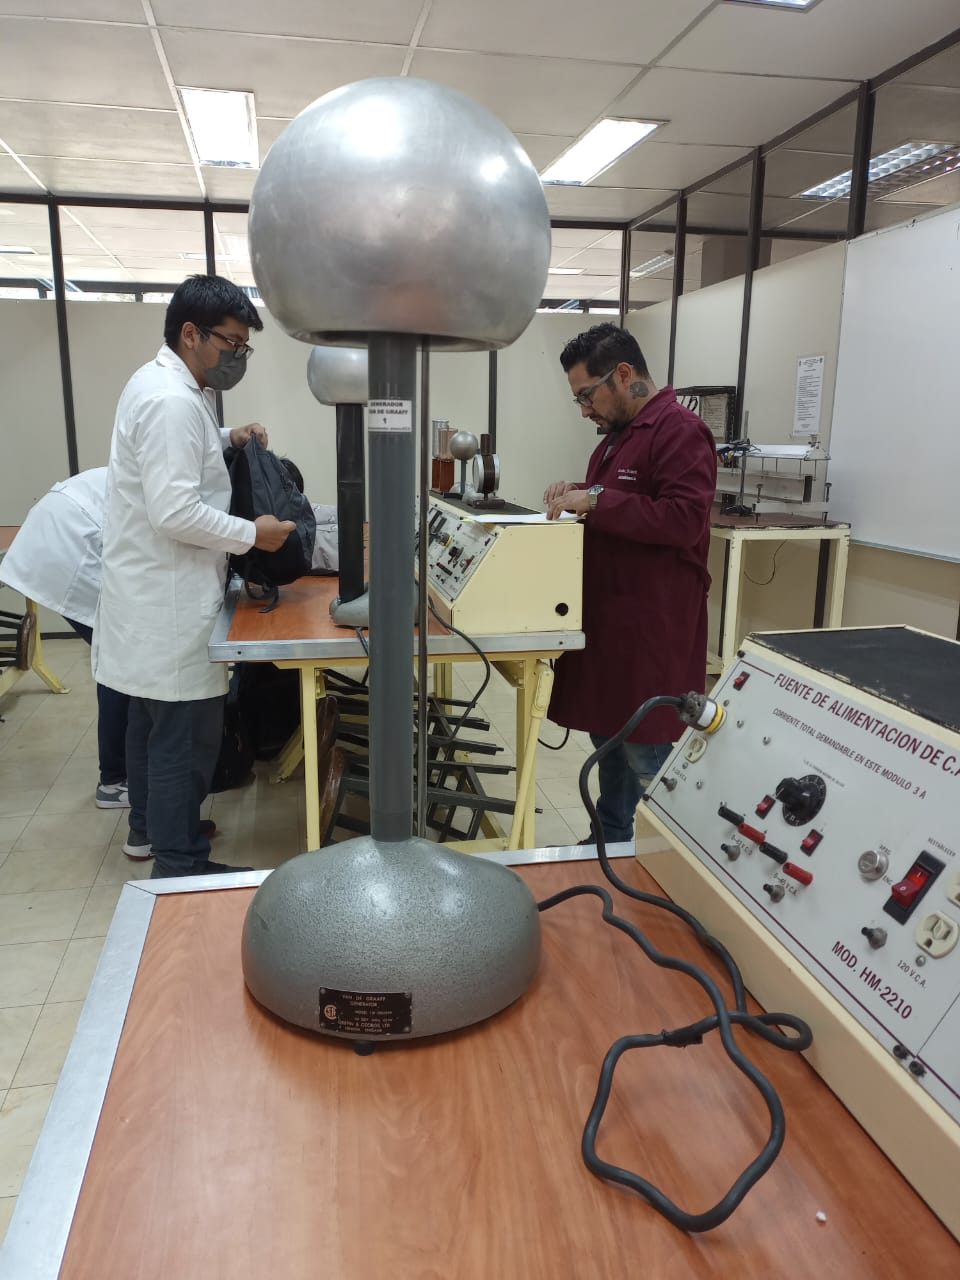
\includegraphics[width=0.1\textwidth]{Vander} 
	
	

Electroscopio: es un instrumento que se utiliza para saber si un cuerpo esta eléctricamente cargado. 

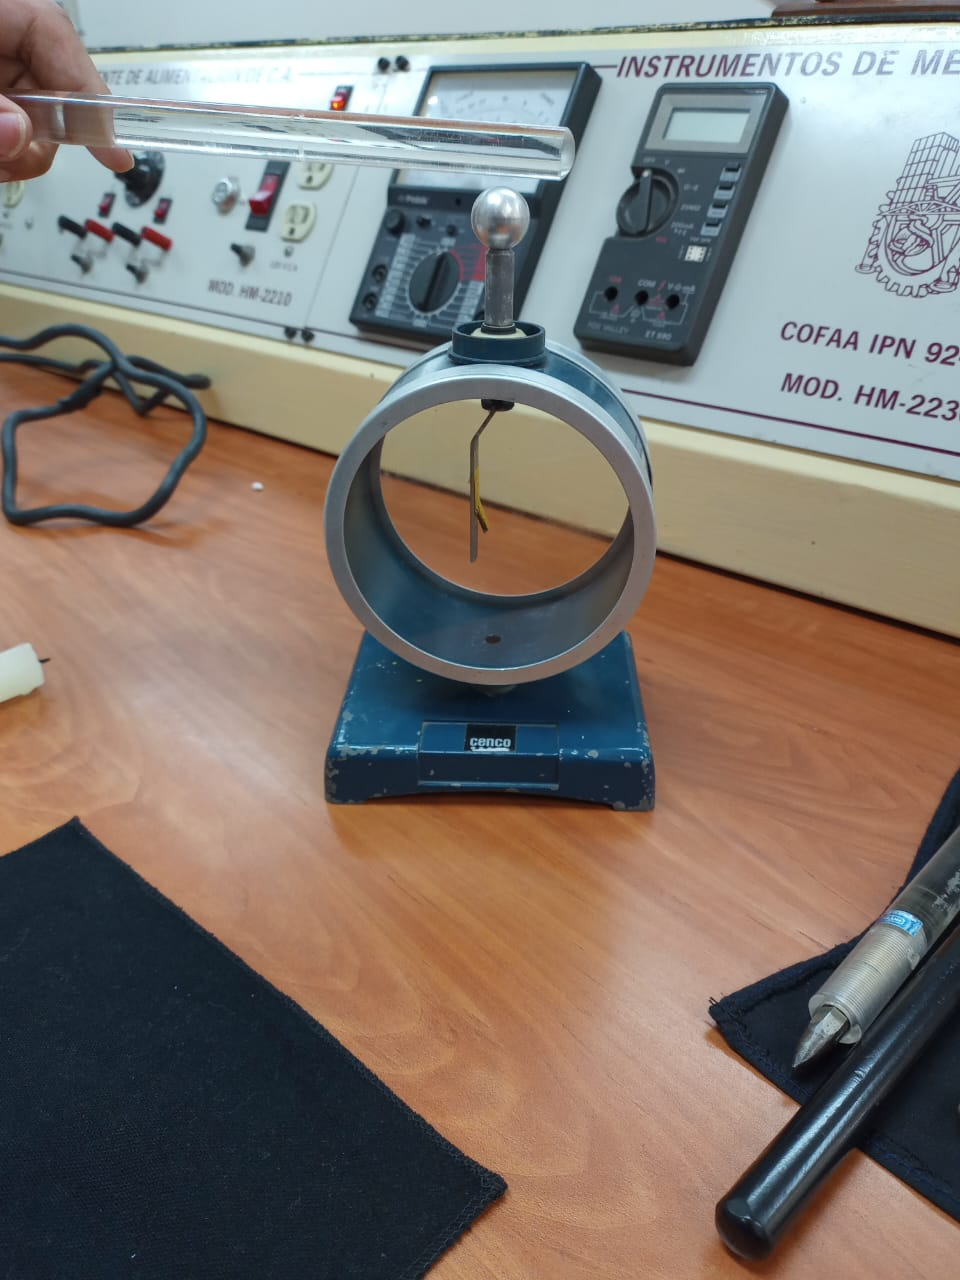
\includegraphics[width=0.1\textwidth]{Metro}

Mechón de cabello y Rehilete electrostático: 
Estos dos instrumentos fueron utilizados para ver la reacción de generador de Van der Graff en base a estos instrumentos y su electrización 

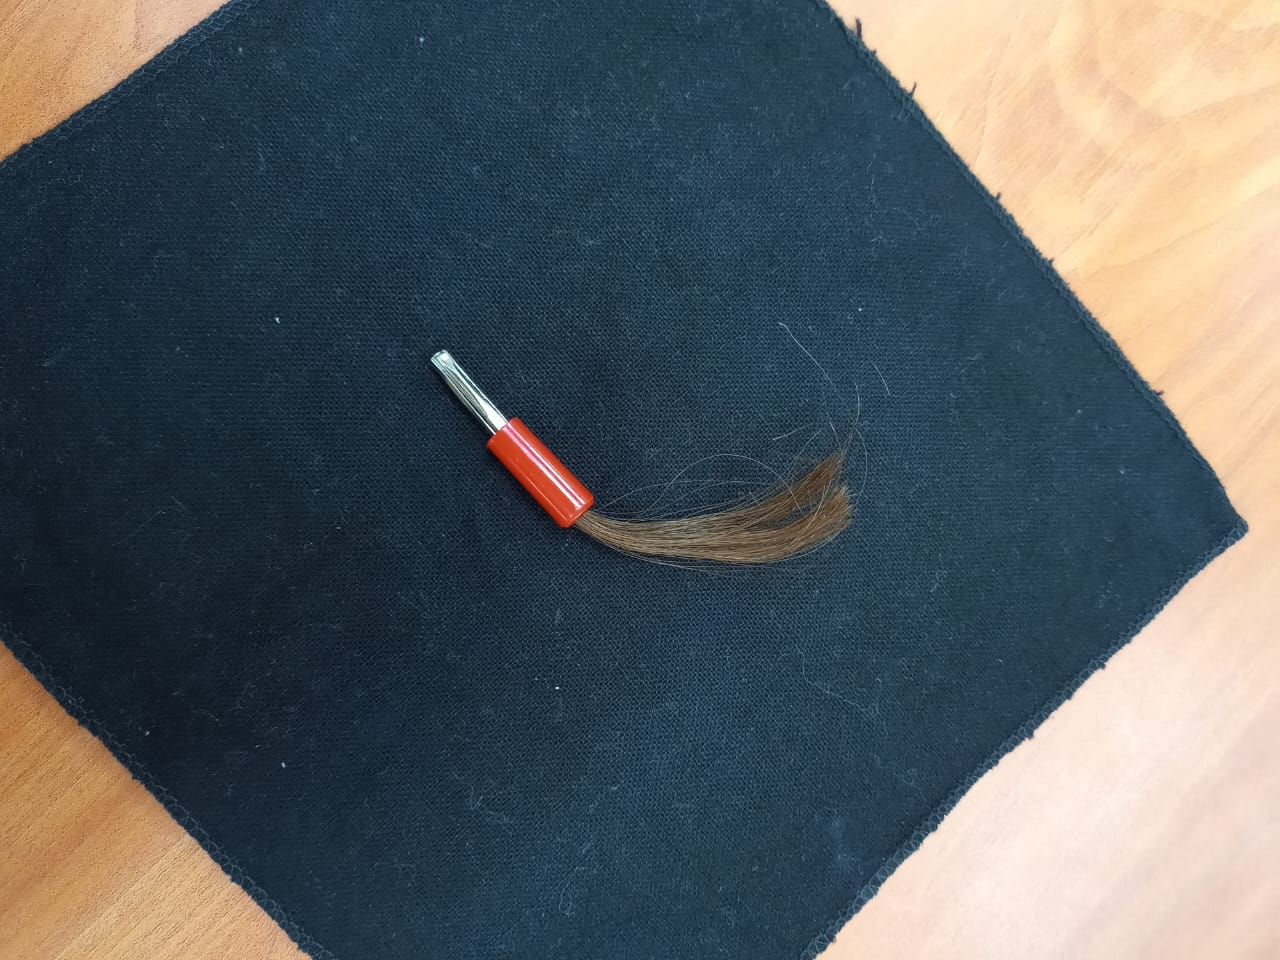
\includegraphics[width=0.1\textwidth]{Pelo}
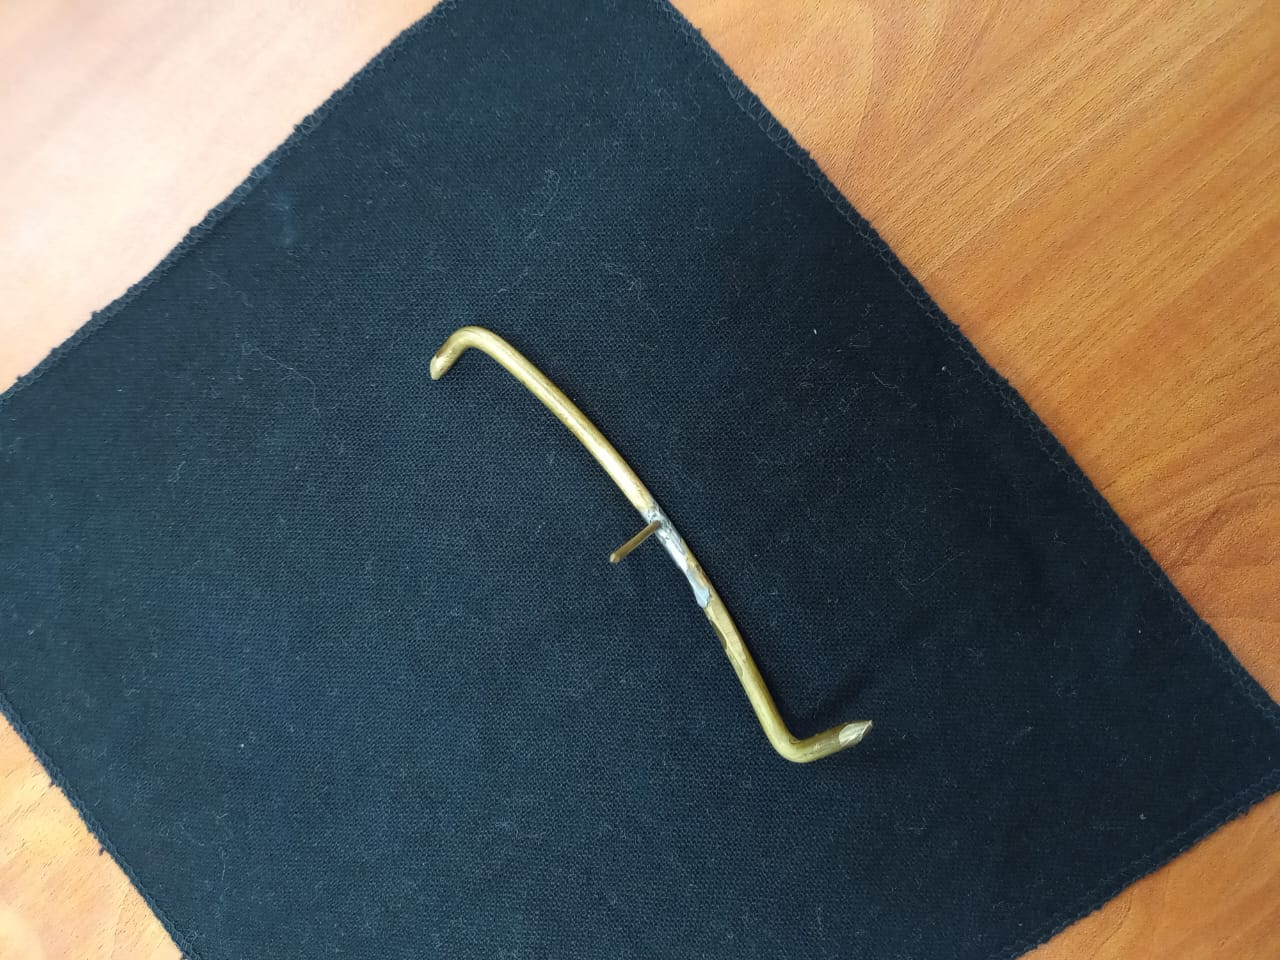
\includegraphics[width=0.1\textwidth]{Rehilete}


Banco aislado, copa de Faraday, recipiente de plástico con esferas de cripsota, esfera hueca, hemisferios de Cavendish
Estos materiales fueron utilizados para entender cómo se puede pasas la electrización de cuerpos con el generador y el electroscopio.

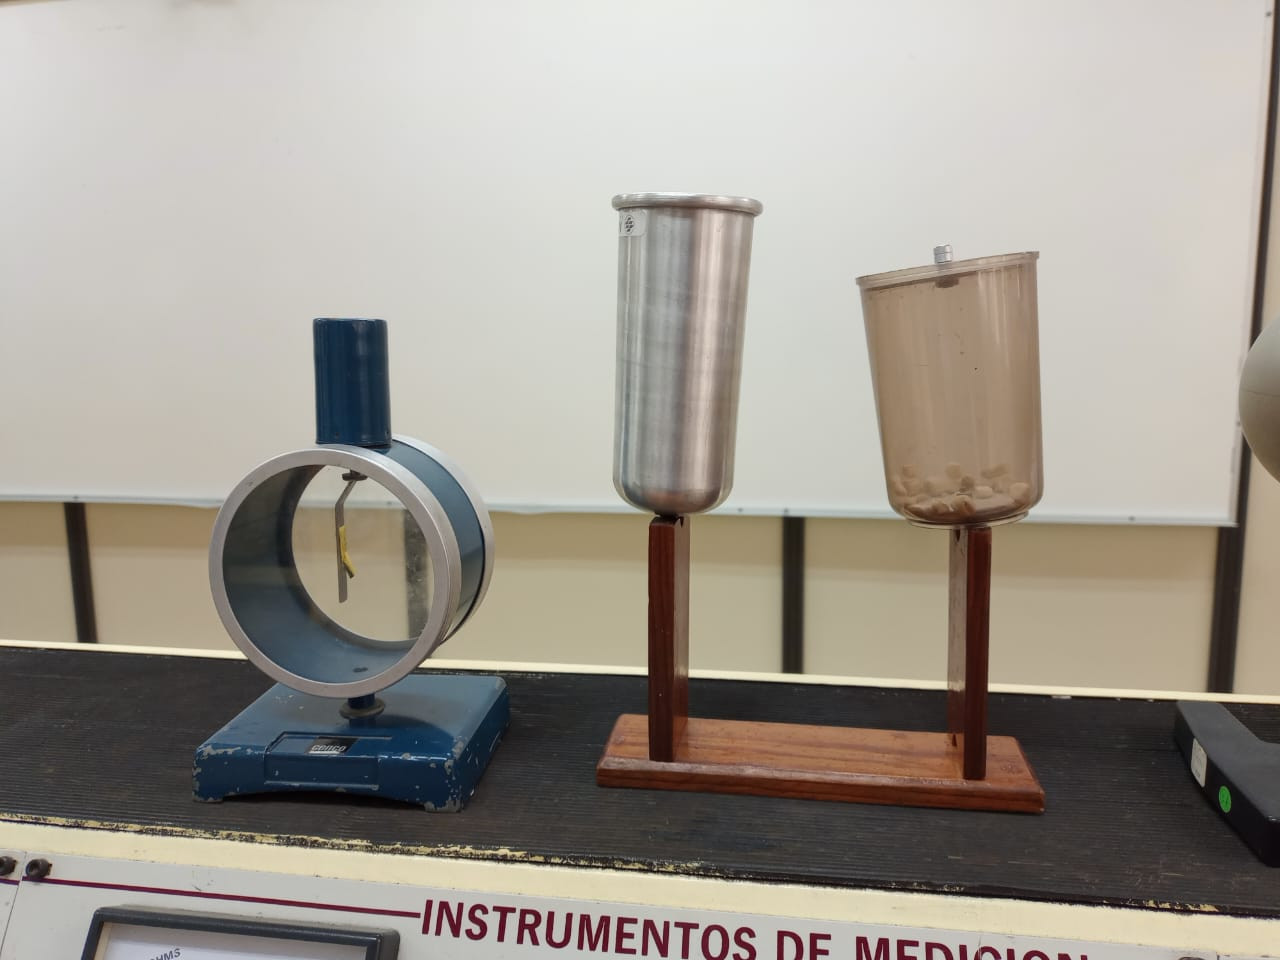
\includegraphics[width=0.1\textwidth]{copas}
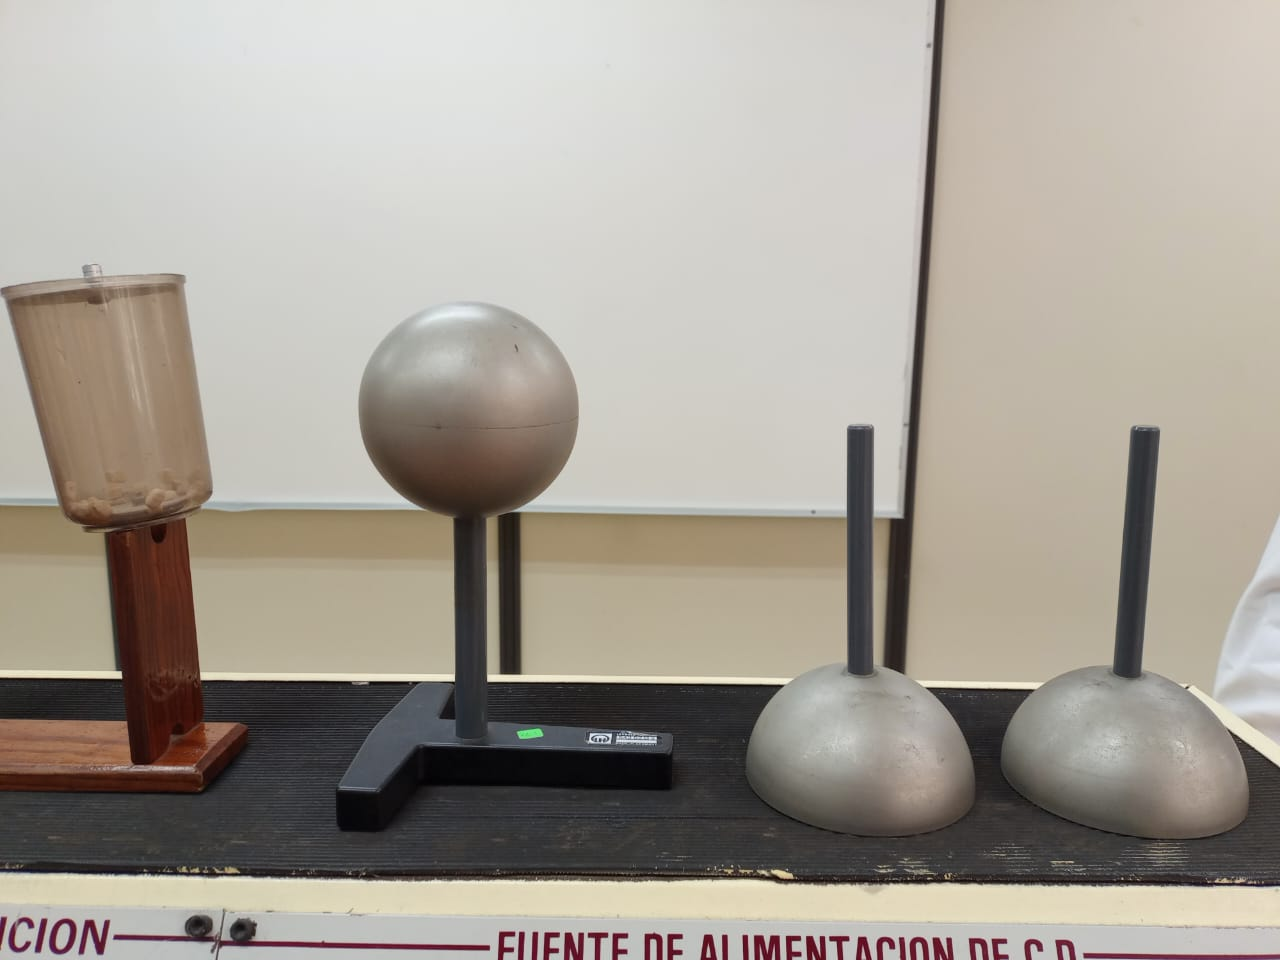
\includegraphics[width=0.1\textwidth]{bolas}

Barra de vidrio, Barra de poliestirena, Electrodo de prueba, paño de lana, paño de seda, punta de metal:
Estos instrumentos funcionaron para entender la electrización por contacto, por fricción y por inducción , a su vez el electrodo de prueba funciono para descargar los demás materiales que quedan con un poco de carga. 

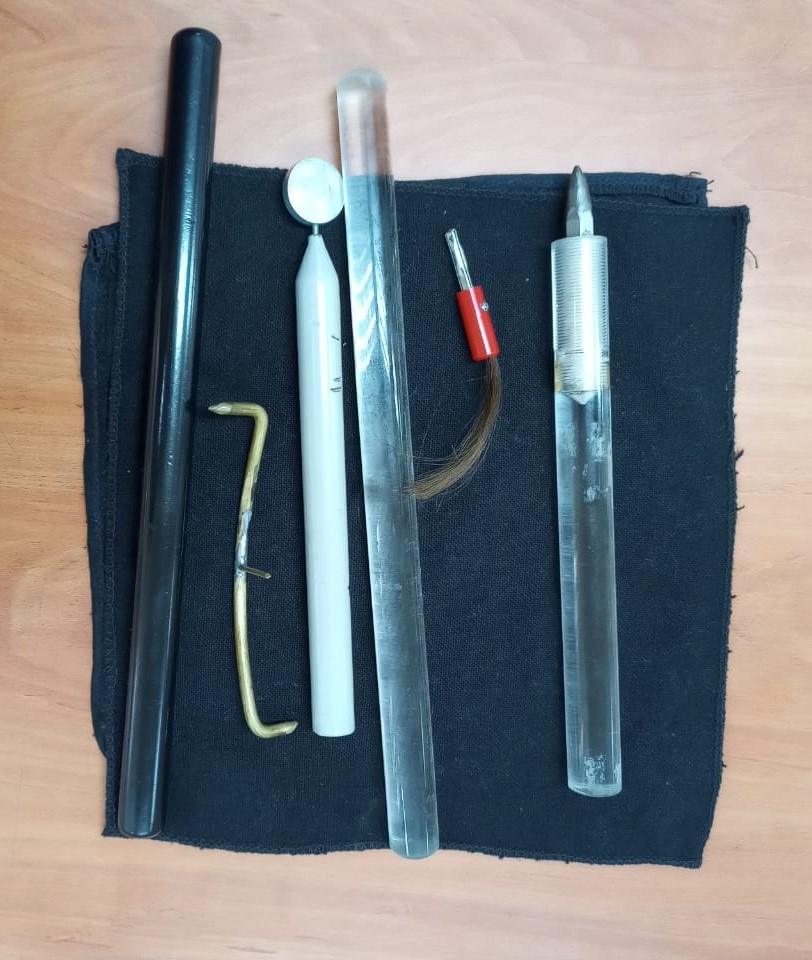
\includegraphics[width=0.1\textwidth]{Herramientas}
\section{Desarrollo experimental.}

\subsection{El electroscopio.}

\subsection{La experiencia de Cavendish.}

\subsection{Experiencia de Franklin.}

\subsection{Pantalla eléctrica.}

\subsection{Efecto de puntas.}

\subsubsection{Rehilete electrostático.}

\subsubsection{Mechón de cabellos.}

\subsubsection{Experiencia de la vela.}



\section{Análisis y resultados.}

\section{Discución.}
Los procesos dados durante la practica son resultados de una serie de acontesimientos y teorias fisicas tales como electrostática, la conductividad, la Ley de Gauss, la densidad superficial de una carga, y conceptos como la jaula de Faraday.Lo cual la suma de todo esto genera que el electroscopio se muevan las pequeñas bolas dentro de los recipientes al igual que estos mismos principios son aplicados en el generador de Vander Graff. 

\section{Conclusiones.}
\subsection{José Emilio Hernández Huerta}
La practica introduce conceptos nuevos los cuales desonocia por completo al igual que nuevas experiencias a la hora de interactuar con el equipo del laboratorio demostrando como el cuerpo humano es un claro conductor al igual que entre mas superficie de contacto alla las cargas se distribuiran de mejor forma esto lo pude notar claramente al poner la lengua cerca del generador de Vander Graff. Pero esto es solo un pequeño acercamiento a lo que nos ofrece el curso, y todo el camino que nos falta pues en algunas practicas nuestras mediciones y observaciones fueron algo erroneas pues haciamos mal los experimentos, siendo que esto influya de manera negativa en nuestro aprendizaje y en nuestros reportes. En sintesis necesitamos mejorar nuestro metodologia de trabajo, aumentar nuestras horas de estudio para comprender mejor el tema y seguir adelante.

\end{multicols}
\newpage
\clearpage
\begin{thebibliography}{0}
	\bibitem{citekey}
\end{thebibliography}

\end{document}